\chapter{Appendix to Chapter 4}
\label{chap:appendix_ch4}

\section{Tuning the Initial Elliptical Slice Sampling Bracket Width}
\label{sec:lna_init_bracket_width}

When fitting SEMs with complex dynamics, e.g., when there are many strata or when the dynamics are time varying, we will be able improve the computational efficiency of our MCMC by initialing the ElliptSS bracket width at $ \omega < 2\pi $. This choice is motivated by the observation that when the model dynamics are complex, the ElliptSS bracket will typically need to be shrunk many times before the sampler reaches a range of acceptable angles in the proposal. Each time we propose a new angle in the ElliptSS algorithm we must solve the LNA ODEs in order to compute the observed data likelihood. Thus, if we can reduce the number of ElliptSS steps, we will be able to shorten the time required to complete our MCMC runs. 

In models where it is advantageous to shring the initial bracket width, we will typically set the initial bracket width to a constant times the standard deviation of the accepted angles in a tuning phase. Since we do not step out the ElliptSS bracket, the initial width should not be so small as to induce additional autocorrelation in the latent process, and should also not be so wide that the bracket is contracted needlessly. We have found a bracket width of $ \omega = 2\sqrt{2\log(10)}\sigma $, corresponding to the full width at one tenth maximum for a Gaussian with standard deviation $ \sigma $, to work well in practice. Figure \ref{fig:esstuning} presents histograms of the number of contractions per ElliptSS update and the accepted angles before and after contracting the initial ElliptSS bracket width for the joint Ebola model of Section \ref{sec:lna_ebola}. In this instance, we were able to substantially reduce the number of contractions, and hence likelihood evaluations, per ElliptSS update while leaving the distribution of accepted angles essentially unchanged. We like to call this a "free lunch".

\begin{figure}
	\centering
	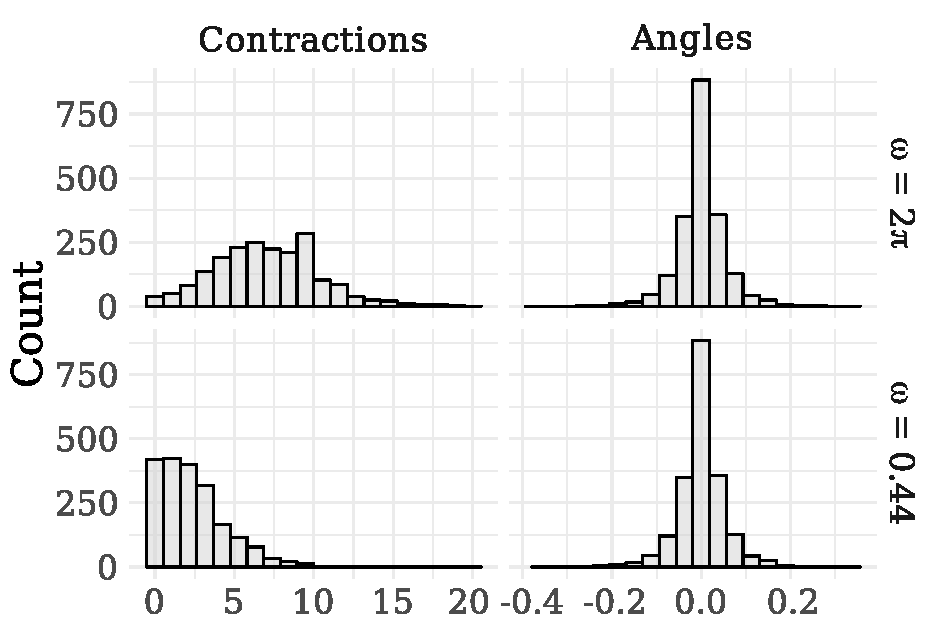
\includegraphics[width=0.7\linewidth]{figures/ess_tuning}
	\caption{Distributions of the numbers of contractions per ElliptSS update and the accepted angles for an MCMC chain for the joint Ebola model of Section \ref{sec:lna_ebola} . An initial bracket width of $ 2\pi $ was used for the first 5,000 iterations (top row), after which the initial bracket width was set to $ 2\sqrt{2\log(10)}\sigma_{ElliptSS} $, where $ \sigma_{ElliptSS} $ was the standard deviation of the accepted angles from the initial run (bottom row).} 
	\label{fig:esstuning}
\end{figure}

We mentioned in Section \ref{subsubsec:noncentered_parameterization} that our ElliptSS algorithm was modified slightly from that presented in \cite{murray2010} in order to facilitate tuning of the initial ElliptSS bracket width. In both cases, the distribution of proposed states, $ \bZ_{prop} $, is centered at the current state $ \bZ_{cur} $. However, the distribution of angles of accepted states using our algorithm will be centered around 0, whereas the distribution of angles for accepted proposals using the algorithm in \cite{murray2010} will be bimodal with peaks at 0 and $ 2\pi $. The algorithms are nevertheless equivalent due to the rotational symmetry of the proposals (a proposal made using an angle $ \phi $ is equivalent to a proposal using $ \phi+2\pi $). It is more natural to compute the standard deviation of the accepted angles if the distribution of angles is symmetric about zero than if it is bimodal (and would thus require a rotation).

\section{Inference for Initial Compartment Volumes}
\label{sec:lna_init_volumes}

When the initial compartment volumes are included as initial parameters in the model instead of being treated as fixed, we will model them as arising from the following truncated multivariate normal distribution: \begin{equation}
\label{eqn:lna_initdist_prior}
\bX_0 \sim TMVN_{\mcS_X^R}(N\bp,N(\bP - \bp\bp^T)),
\end{equation} 
where $ \bp $ is a vector of subject--level initial state probabilities, $ \bP = \diag(\bp) $, $ N $ is the population size, and the subscript $ \mcS_X^R $ specifies the state space of $ \bX $ (so that the compartment volumes add up to $ N $ and each compartment volume is non--negative and less than the total population size at time $ t_0 $). Thus, the initial distribution is specified as the truncated normal approximation of a multinomial distribution with size $ N $ and probability vector $ \bp $. In models with multiple strata, we will similarly model the initial compartment volumes as having independent truncated multivariate normal distributions that are each approximations of multinomial distributions over initial compartment counts within each stratum. Notation and details are completely analogous to the single stratum case, and are therefore omitted for the sake of clarity.

Let $ \bV = N(\bP - \bp\bp^T) $, and $ \bV^{1/2} $ be the matrix square root of $ \bV $, which we will compute using the singular value decomposition $ \bV = \bU\bD\bU^T \implies \bV^{1/2} = \bU\bD^{1/2}$. Let $ \bZ^X $ denote the LNA draws as before, and let $ \bZ^{X_0}\sim\mr{MVN}(\bs{0},\mb{I}) $ denote the vector of draws that will be mapped to $ \bX_0 $. We will update the initial compartment volumes jointly with the LNA draws using elliptical slice sampling.

\begin{algorithm}[!ht]
	\caption{Sampling LNA draws and initial volumes via elliptical slice sampling.}
	\label{alg:elliptss_lna_initvols}
	\begin{algorithmic}[1]
		\Procedure{\doElliptSS2}{$ \bZ^X_{cur}, \bZ^{X_0}_{cur},\btheta,\bY,\mcI,\omega = 2\pi $}
		\State Sample ellipse: $ \bZ^X_{prop} \sim N(\bs{0}, \mb{I}),\ \bZ^{X_0}_{prop} \sim N(\bs{0}, \mb{I})$
		\State Sample threshold: $ u|\bx \sim \mr{Unif}(0, L(\bY|\doLNA(\bZ_{cur},\btheta,\mcI))) $
		\State Position the bracket and make initial proposal: \vspace{-0.1in}
		\begin{align*}
		\psi &\sim \mr{Unif}(0,\omega)\\
		L_\psi &\leftarrow -\psi;\ R_\psi \leftarrow L_\psi + \psi\\
		\phi &\sim \mr{Unif}(L_\psi,R_\psi)
		\end{align*}
		\State Set $ \bZ^{X'} \leftarrow \bZ^X_{cur}\cos(\phi) + \bZ^X_{prop}\sin(\phi) $, $ \bX_0^\prime = \bV^{1/2}\left (\bZ^{X_0}_{cur}\cos(\phi) + \bZ^{X_0}_{prop}\sin(\phi)\right ) $ 
		\If{$ L(\bY|\doLNA(\bZ',\btheta^\prime,\mcI)) > u $}{ accept $ \bZ^{X^\prime},\bZ^{X_0^\prime} $}
		\State\Return{ $ \bZ' $}
		\Else
		\State Shrink bracket and try a new angle:
		\State{\textbf{If:} $ \phi < 0 $}{ \textbf{then: }$ L_\phi \leftarrow\phi $ }{ \textbf{else: }$ R_\phi \leftarrow \phi $}
		\State $ \phi \sim \mr{Unif}(L_\phi, R_\phi) $
		\State \textbf{GoTo:} 5
		\EndIf
		\EndProcedure
	\end{algorithmic}
\end{algorithm}

\section{Choice of Estimation Scale and Implications for Mixing and Convergence}
\label{sec:est_scale_discussion}

How we parameterize the MCMC estimation scale is critically important to its computational performance. If we can identify transformations of the model parameters that minimize strong correlations and non--linear relationships on the estimation scale, we will be able to substantially improve MCMC mixing. In our context, it will often be relatively straightforward to identify such transformations (or at least intermediate transformations that can be used in combination). As a general approach, we will try to identify transformations that reflect the ways in which model parameters jointly act on the model dynamics, and then a second set of transformations that remove any boundary conditions. 

As an example, consider the single country SEIR model fit to the incidence data from Sierra Leone in Section \ref{sec:lna_ebola}. This model includes parameters for the external force of infection and the effective population size, which add complexity to the usual formulation of the SEIR dynamics as being entirely driven by endogenous contacts within a closed homogeneously mixing population. The model parameters on their natural scales are provided in Table \ref{tab:seir_params_nat}. Each of the model parameters has a clear marginal interpretation, but upon examining the pairwise scatterplots of the posterior (Figure \ref{fig:slpairs1}) it becomes obvious that the parameters interact in highly non--linear ways. We would encounter a variety of pathological computational problems if we were to naively parameterize the MCMC estimation scale without considering the ways in which the parameters interact to affect the dynamics. For example, it would be extremely difficult for any sampler that does not account for the curvature in the posterior, e.g., Hamiltonian Monte Carlo (HMC), to explore the parameter space. (An aside: we experimented with implementing the LNA in \texttt{Stan} and using HMC to sample the posterior, but repeatedly integrating the LNA ODEs along with their augmented sensitivity equations was prohibitively slow for even simple models).  

\begin{table}[!ht]
	\label{tab:seir_params_nat}
	\caption{SEIR model parameter and their interpretation on their natural scales.}
	\footnotesize
	\centering
	\begin{tabular}{clc}
		\textbf{Parameter} & \textbf{Interpretation} & \textbf{Domain}\\
		\hline
		$\alpha$ & Rate of infectious contact from outside the population & $[ 0,\infty) $ \\
		$ \beta $ & Per--contact rate of infection within the population & $[0,\infty) $\\
		$ \omega $ & Rate of transition from $ E\rightarrow I $ & $[ 0,\infty) $\\
		$ \mu $ & Rate of transition from $ I\rightarrow R $ & $[ 0,\infty) $\\
		$ \rho $ & Mean case detection probability & $[ 0,1] $\\
		$ \phi $ & Negative binomial overdispersion parameter & $[ 0,\infty) $ \\
		$ N_{eff} $ & Effective population size & $[0,N]$\\
		\hline
	\end{tabular}
\end{table}

\begin{figure}[!ht]
	\centering
	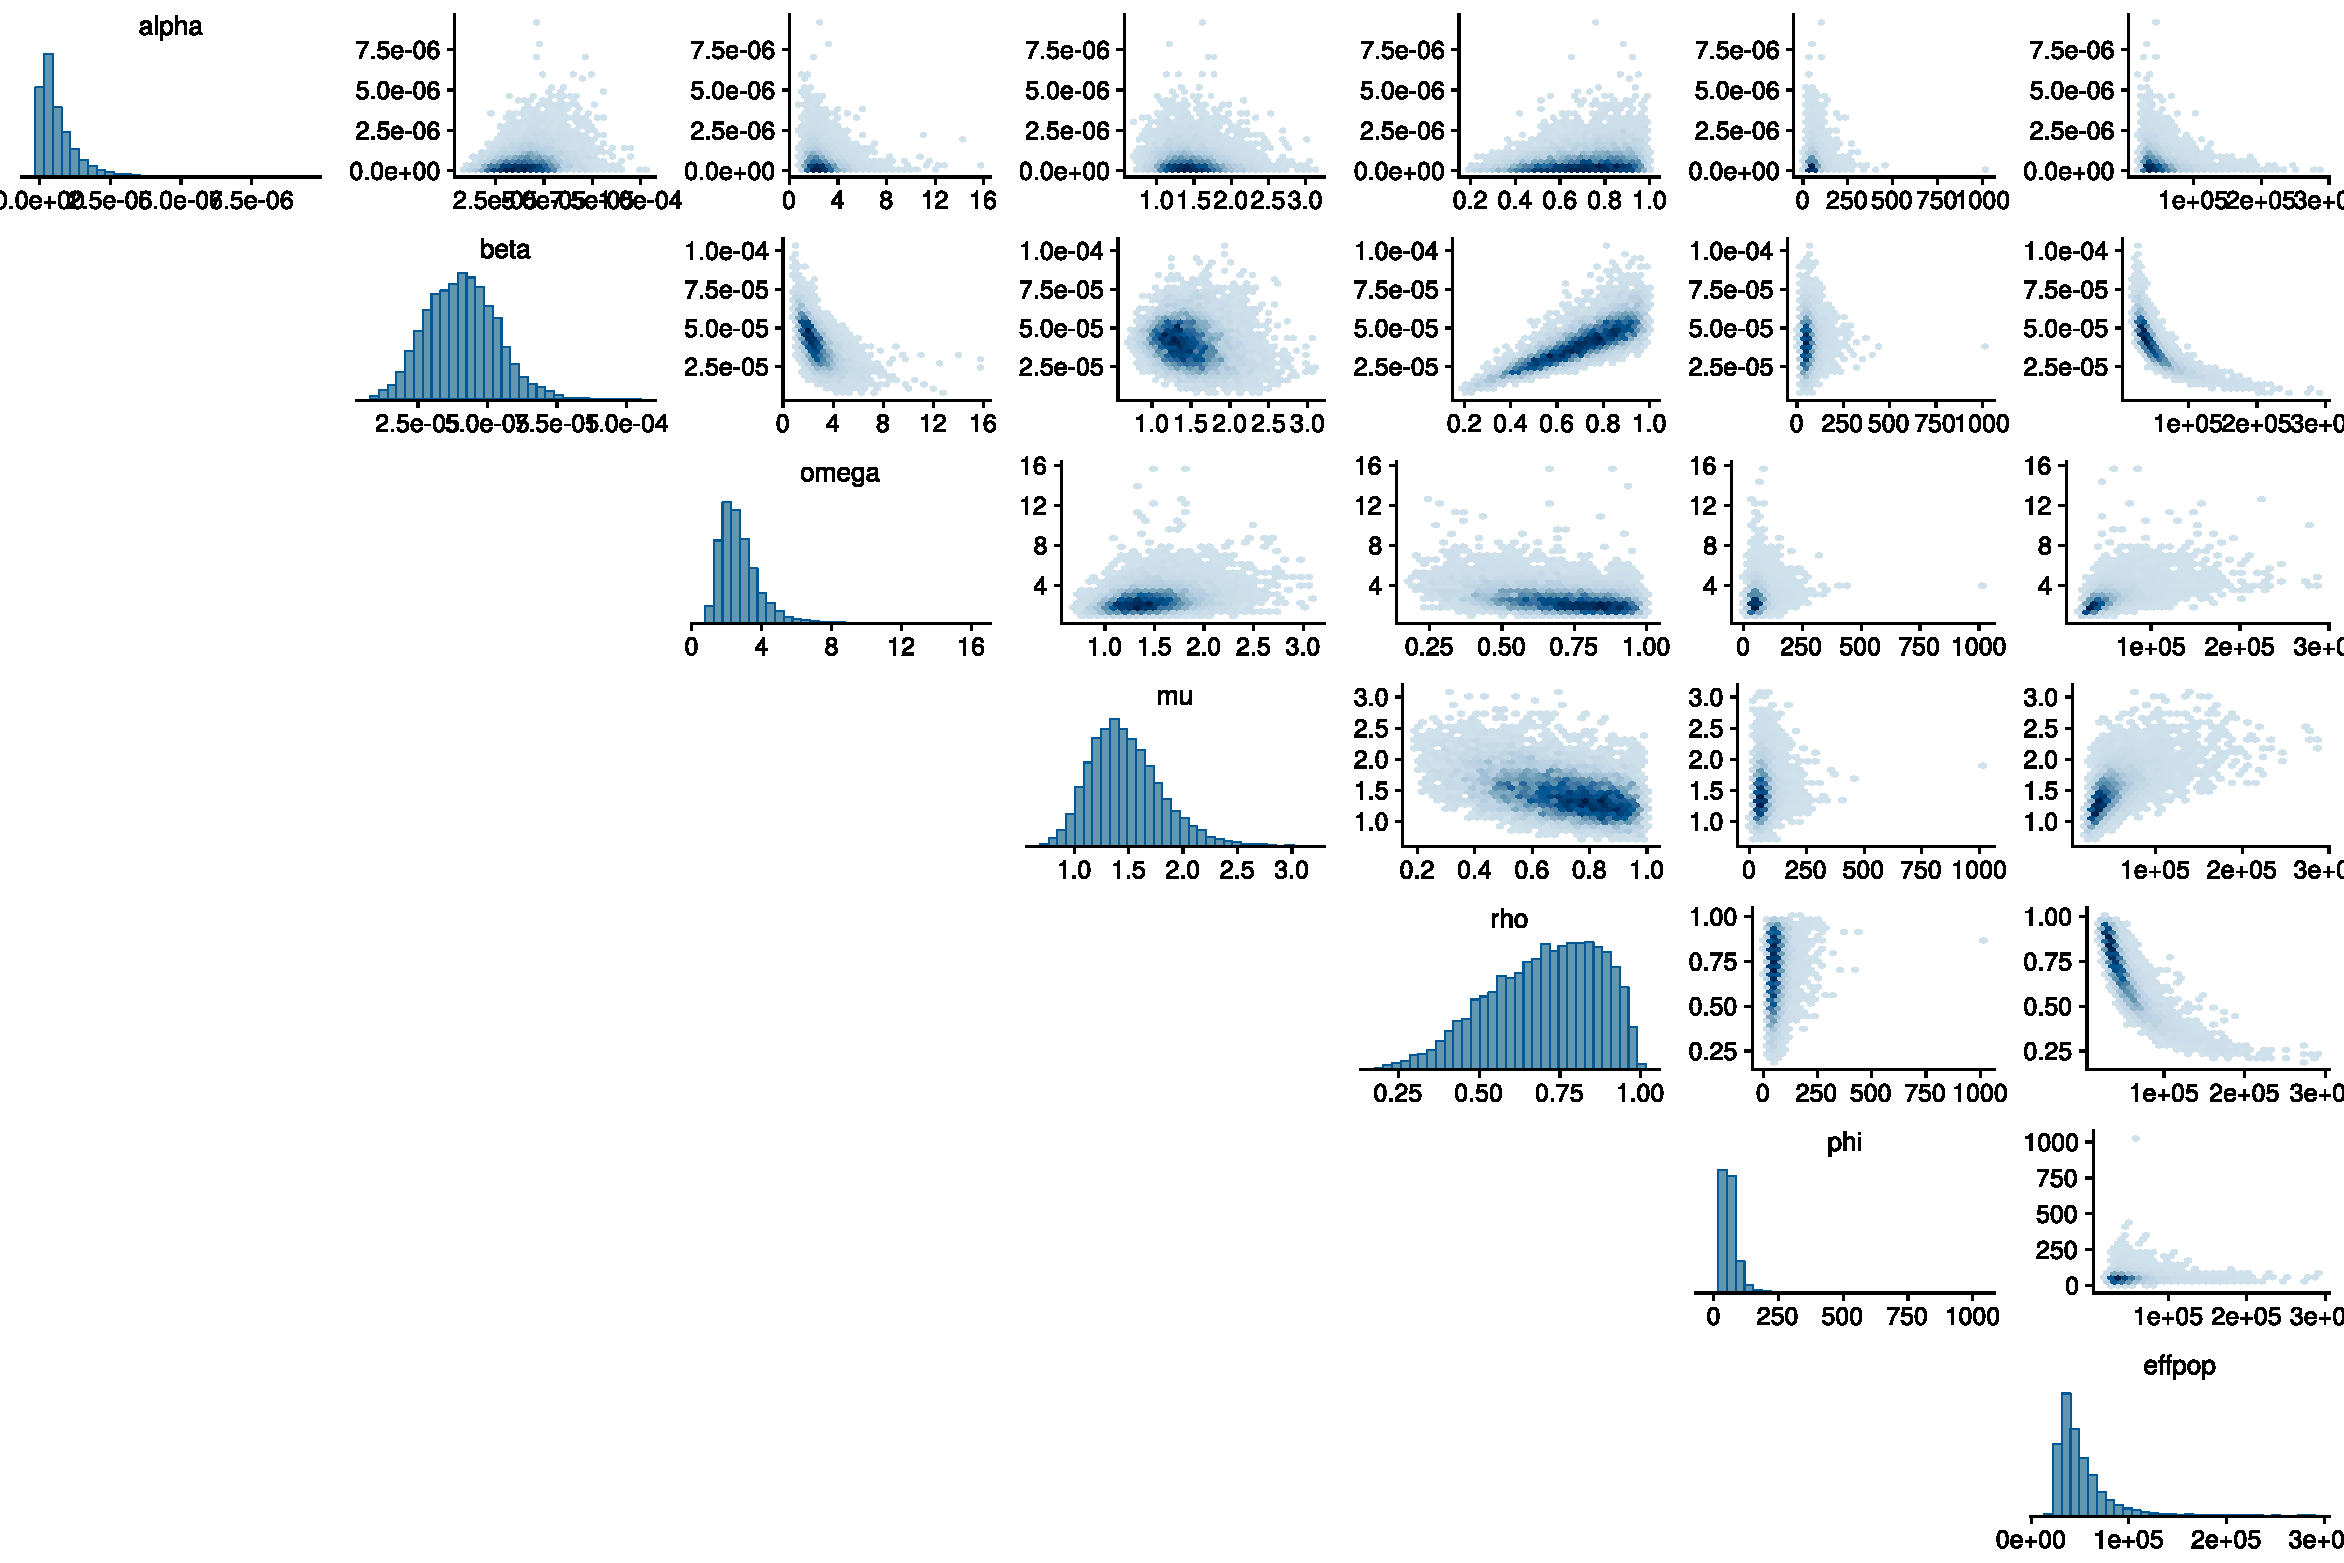
\includegraphics[width=\linewidth]{figures/sl_pairs_1}
	\caption{Marginal histograms and pairwise scatterplots of posterior samples for parameters for the SEIR model fit to the Sierra Leone Ebola dataset using the estimation scale in Table \ref{tab:seir_params_est3}. The parameters on the estimation scales in this figure and their interpretations are provided in Table \ref{tab:seir_params_nat}.} 
	\label{fig:slpairs1}
\end{figure}

We can mitigate the problems caused by non--linear relationships and strong correlations among parameters by parameterizing the estimation scale in terms of how the parameters jointly affect the model dynamics and then removing the boundary conditions. Table \ref{tab:seir_params_est2} provides a list of parameters on their estimation scale that are reflective of an initial first pass at how we would expect the parameters to interact. For example, the parameters governing the rates of infectious contact, $ \alpha$ and $\beta $, combine with the effective population size and the infectious period duration to produce the basic reproductive numbers with respect to initially infected individuals outside and inside the population. Still, we can see that there are some residual non--linear relationships between the log effective population size, the logit case detection probability, and the effective reproductive number. If we were to use this parameterization, we might survive the computational difficulties that the previous parameterization presented, at least for this dataset. The analogous model fit to the data from Liberia using this parameterization would (and did) struggle mightily. We can see in Figure \ref{fig:libpairs2} that this parameterization still results in non--linear relationships in the posterior for the model fit to the Liberia dataset. 

\begin{table}[!ht]
	\label{tab:seir_params_est2}
	\caption{SEIR model parameter and their interpretation on a possible set of estimation scales.}
	\footnotesize
	\centering
	\begin{tabular}{clc}
		\textbf{Parameter} & \textbf{Interpretation} & \textbf{Domain}\\
		\hline
		$\log(R_{eff}^{ext}) = \log(\alpha N_{eff} / \mu)$ & \makecell[l]{Log basic reproductive number given an infected \\outside the population} & $(-\infty,\infty) $ \\
		$ \log(R_{eff} - 1) = \log(\beta N_{eff}/\mu - 1) $ & \makecell[l]{Log basic reproductive number given an infected\\ inside the population and $ R_{eff} > 1 $.} & $(-\infty,\infty) $\\
		$ \log(1/\omega) $ & Log mean latent period duration & $(-\infty,\infty) $\\
		$ \log(1/\mu) $ & Log mean infectious period duration & $ (-\infty,\infty) $\\
		$ \logit(\rho) $ & Logit mean case detection probability & $(-\infty,\infty) $\\
		$ \log(\phi) $ & Log negative binomial overdispersion parameter & $ (-\infty,\infty) $ \\
		$ \log(N_{eff}) $ & Log effective population size & $(-\infty,\log(N))$\\
		\hline
	\end{tabular}
\end{table}

\begin{figure}[!ht]
	\centering
	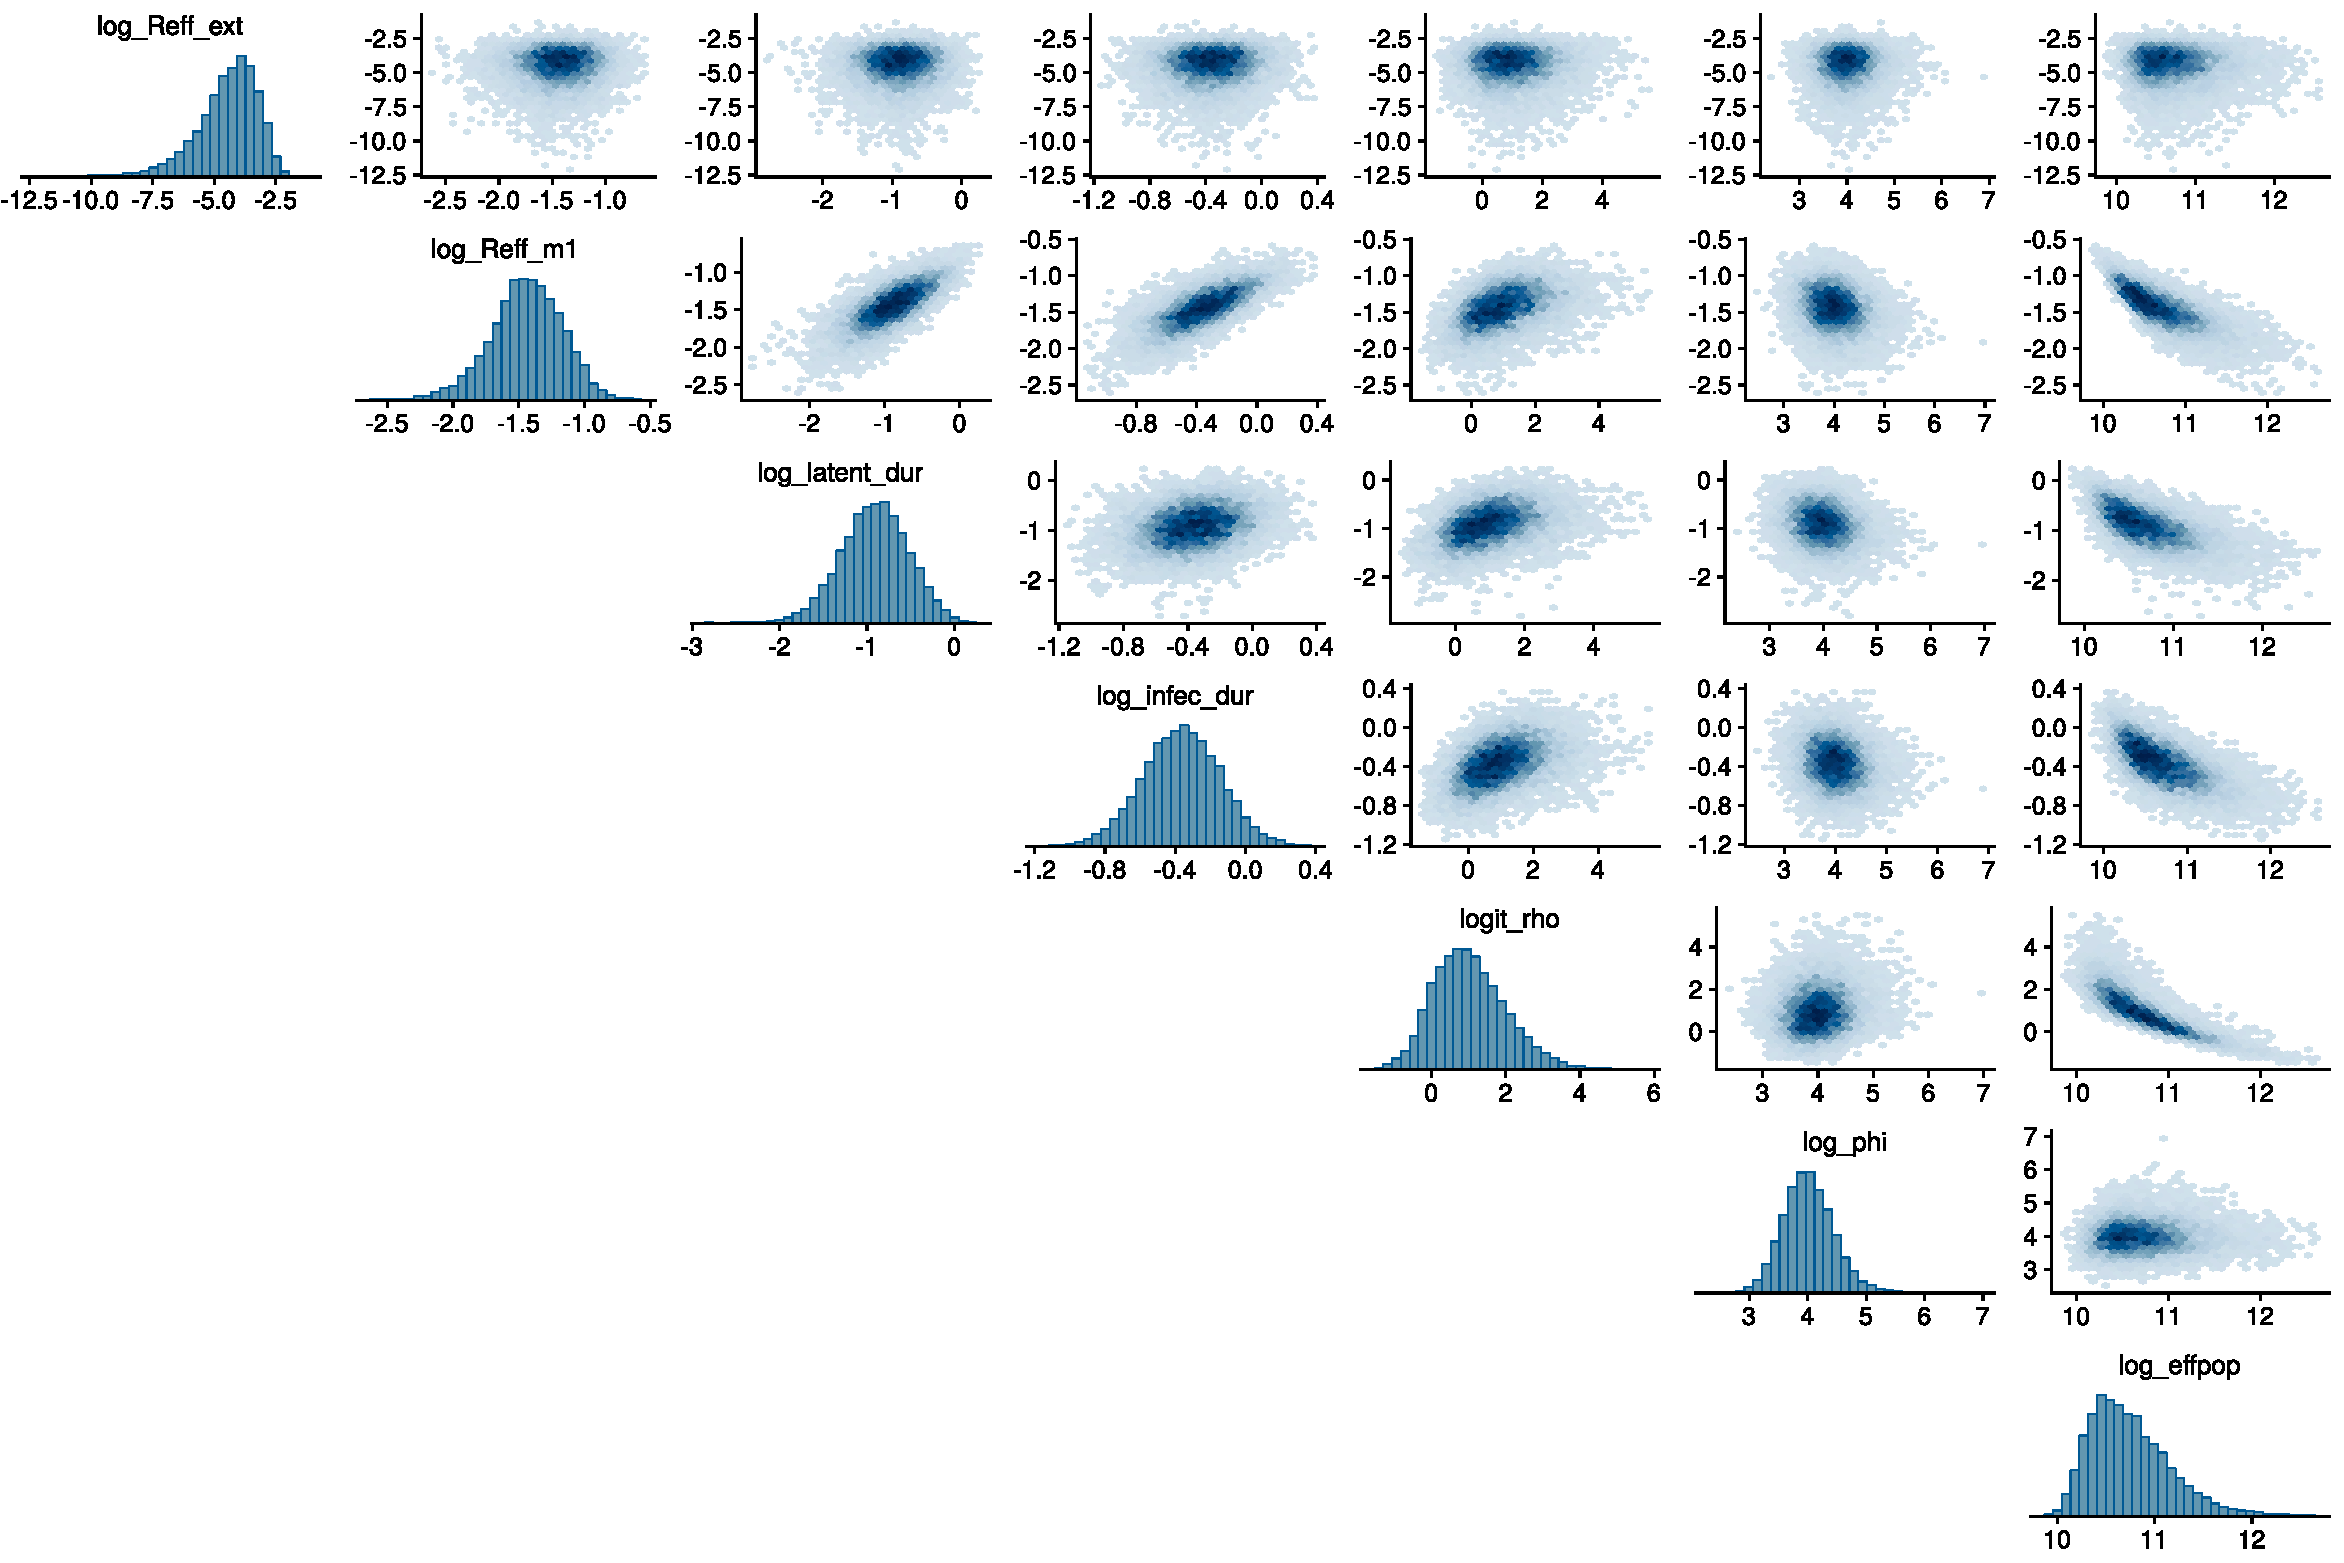
\includegraphics[width=\linewidth]{figures/sl_pairs_2}
	\caption{Marginal histograms and pairwise scatterplots of posterior samples for parameters for the SEIR model fit to the Sierra Leone Ebola dataset using the estimation scale in Table \ref{tab:seir_params_est3}. The parameters on the estimation scales in this figure and their interpretations are provided in Table \ref{tab:seir_params_est2}.} 
	\label{fig:slpairs2}
\end{figure}

\begin{figure}[!ht]
	\centering
	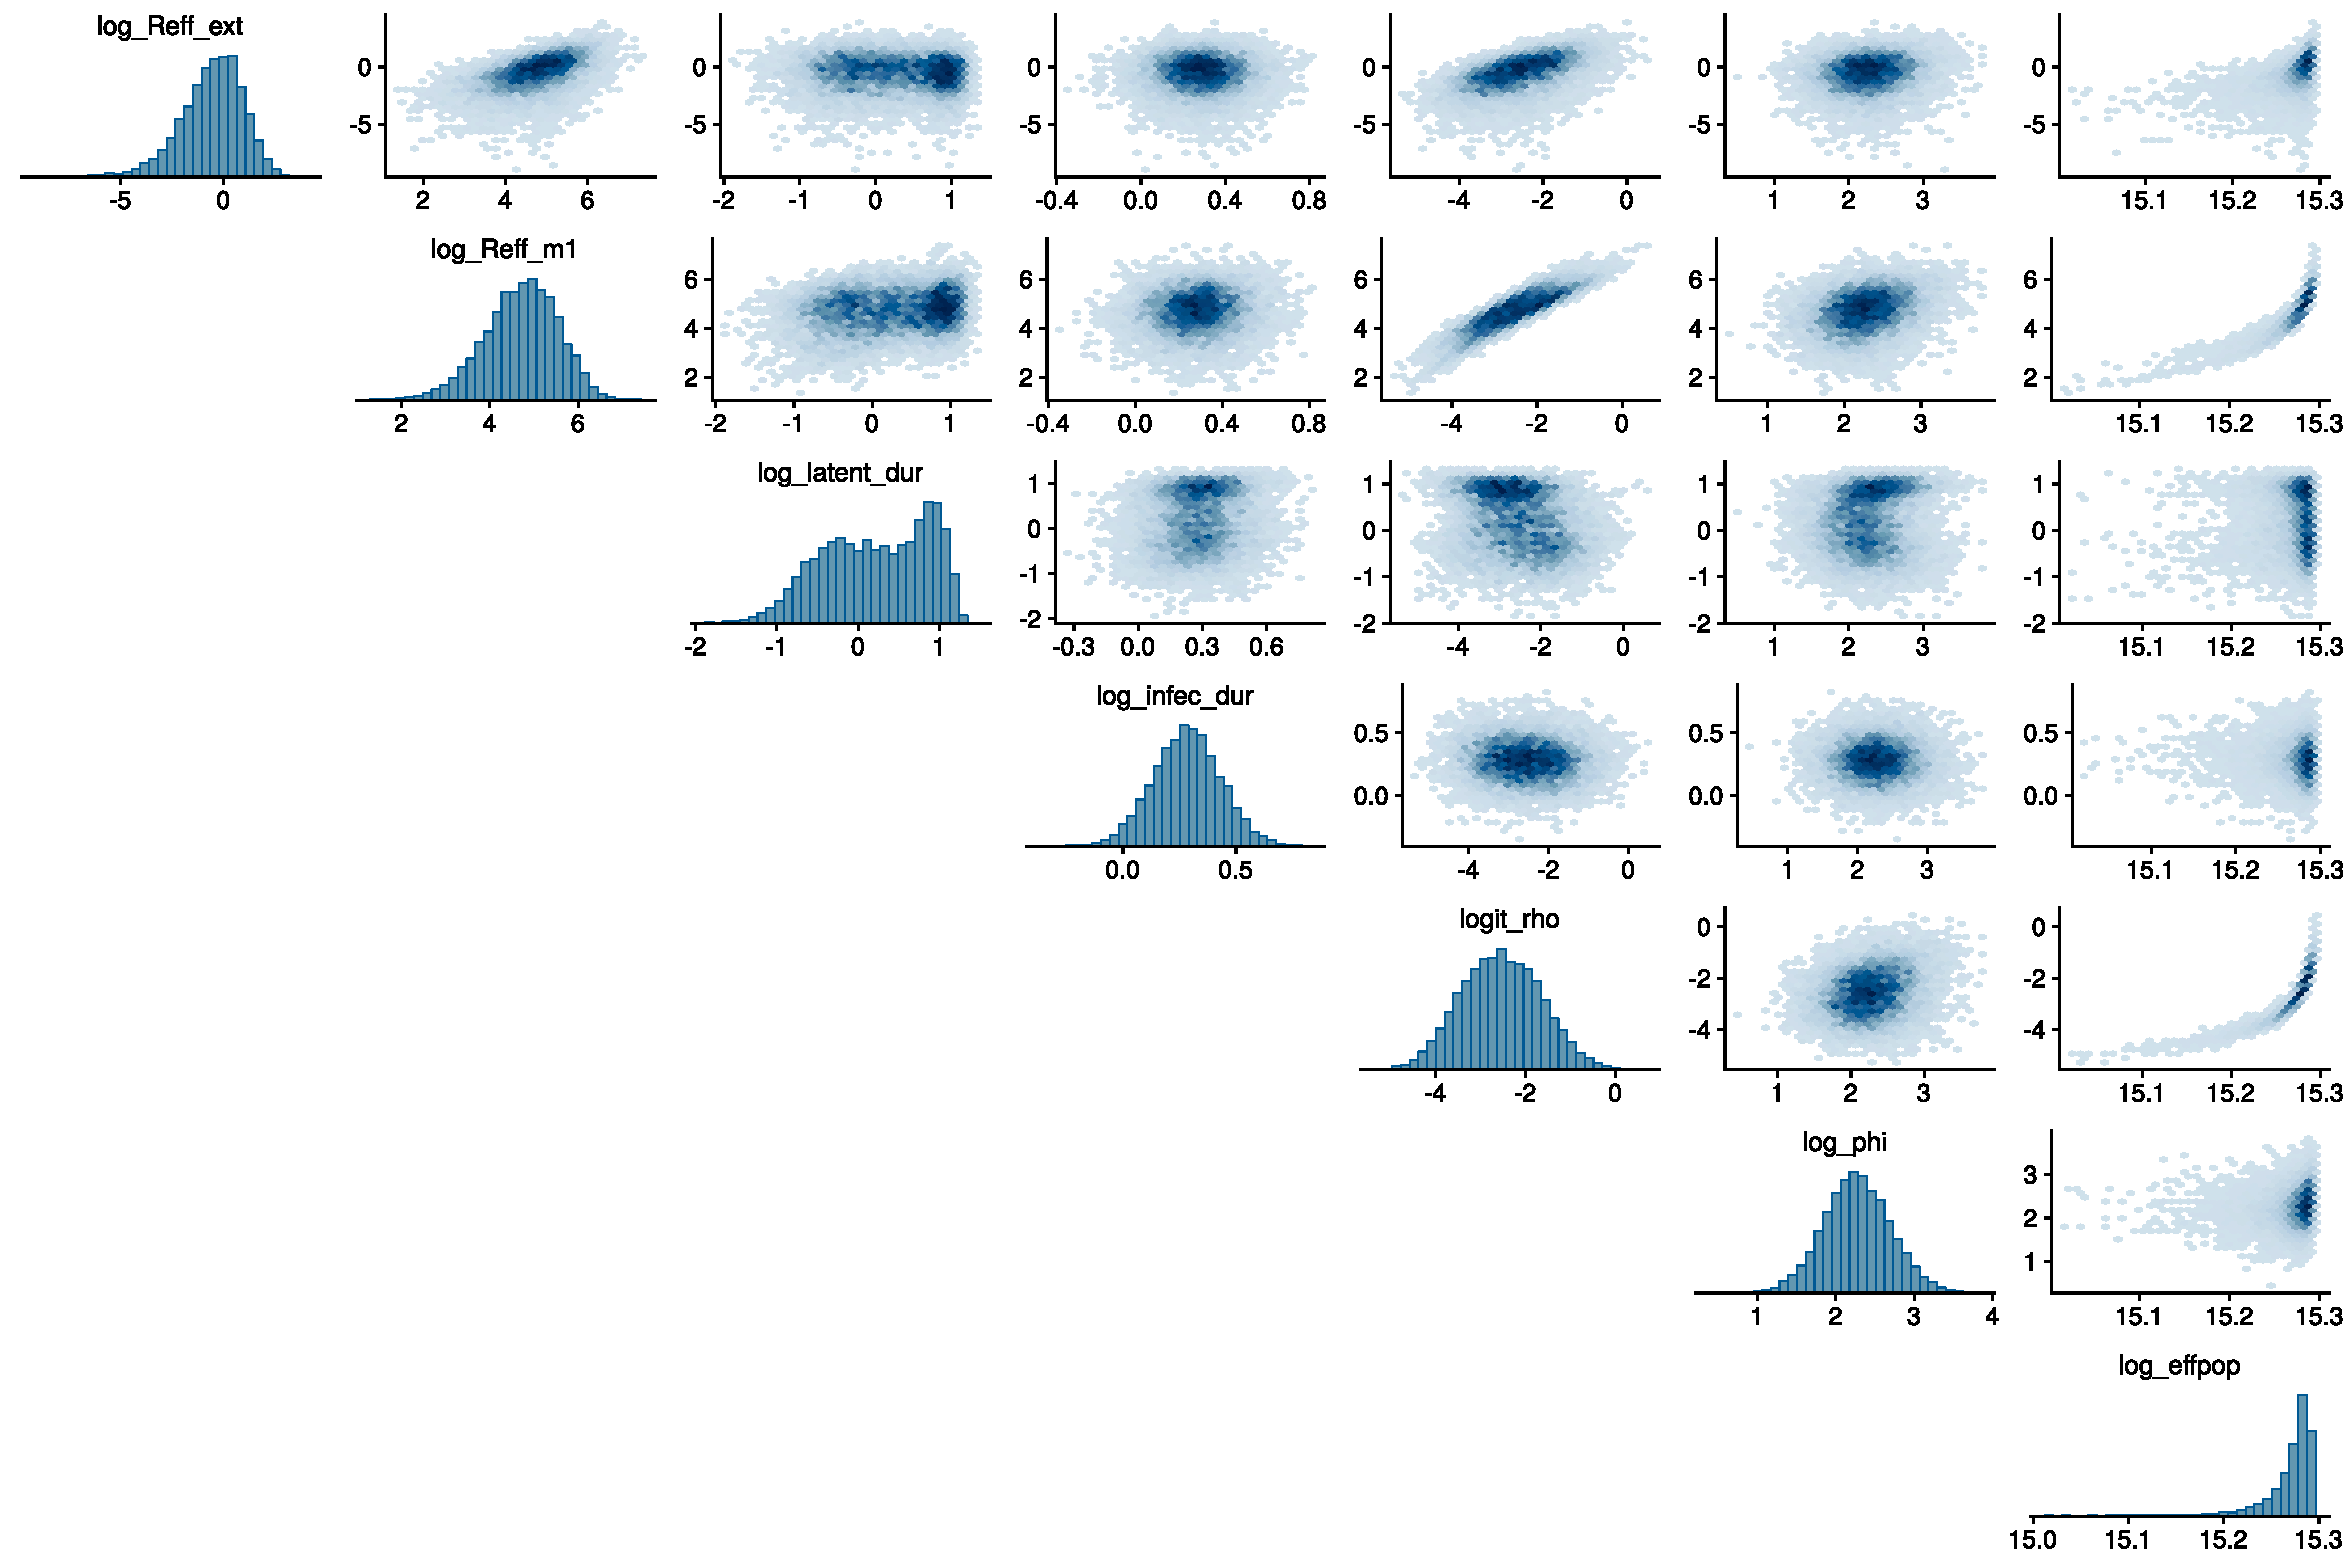
\includegraphics[width=\linewidth]{figures/lib_pairs_est2}
	\caption{Marginal histograms and pairwise scatterplots of posterior samples for parameters for the SEIR model fit to the Liberia Ebola dataset using the estimation scale in Table \ref{tab:seir_params_est2}. The parameters on the estimation scales in this figure and their interpretations are provided in Table \ref{tab:seir_params_est2}.} 
	\label{fig:libpairs2}
\end{figure}

It behooves us to consider how the previous functions of model parameters interact within the model. The effective population size, on its own, in this model is essentially a nuisance parameter. However, combined with the mean case detection probability, the mean case detection rate, $ \rho N_{eff} $ should be, more or less, on the same scale as the total number of observed cases modulo the fraction of the effective population to escape infection. We note that estimation of this quantity is stable even when the population size is misspecified, see, e.g., \cite{fintzi2017efficient, koepke2016predictive}. Moreover, we should suspect, \textit{a priori}, that the basic reproductive number interacts with the mean case detection rate. To understand this, we examine how the basic reproductive number acts on the outbreak size through the final size relation for the deterministic ODE analog to our model \cite{bauer2008compartmental}: 
\begin{equation}
\label{eqn:final_size_relation}
\log\frac{S_0}{S_\infty} = R0\left (1 - \frac{S_\infty}{N}\right ).
\end{equation}
This equation relates the fraction of the population that eventually becomes infected with the basic reproductive number. As $ R0 $ increases, a larger fraction of the population becomes infected. If the effective population size is large, and if the $ R0 $ is high, the mean case detection probability should be low so that the mean case detection rate is concordant with the scale of the observed counts. This is all to suggest that the combination of parameters that jointly acts on the model is the effective reproductive number, offset by the mean case detection rate. The other reparameterization we suggest is to use the infectious period duration and the ratio of the latent to infectious period durations. The new estimation scale is given in Table \ref{tab:seir_params_est3}. On this estimation scale, the posterior for Sierra Leone is much better behaved, with weaker pairwise correlations and very little in the way of non--linear relationships between the model parameters. Similarly, the posterior for Liberia is substantially less pathological. 

\begin{table}[!ht]
	\label{tab:seir_params_est3}
	\caption{SEIR model parameter and their interpretation on a possible set of estimation scales.}
	\footnotesize
	\centering
	\begin{tabular}{clc}
		\textbf{Parameter} & \textbf{Interpretation} & \textbf{Domain}\\
		\hline
		$\log(R_{eff}^{ext}) = \log(\alpha N_{eff} / \mu)$ & \makecell[l]{Log basic reproductive number given an infected \\outside the population} & $(-\infty,\infty) $ \\
		$ \log(R_{eff} - 1) + \log(\rho N_{eff}) $ & \makecell[l]{Log basic reproductive number given an infected\\ inside the population and $ R_{eff} > 1 $, offset\\ by the mean case detection rate} & $(-\infty,\infty) $\\
		$ \log(\omega/\mu) $ & Log ratio of mean latent to infectious period durations & $(-\infty,\infty) $\\
		$ \log(1/\mu) $ & Log mean infectious period duration & $ (-\infty,\infty) $\\
		$ \logit(\rho) $ & Logit mean case detection probability & $(-\infty,\infty) $\\
		$ \log(\phi) $ & Log negative binomial overdispersion parameter & $ (-\infty,\infty) $ \\
		$ \log(\rho N_{eff}) $ & Log mean case detection rate & $(-\infty,\log(N))$\\
		\hline
	\end{tabular}
\end{table}

\begin{figure}[!ht]
	\centering
	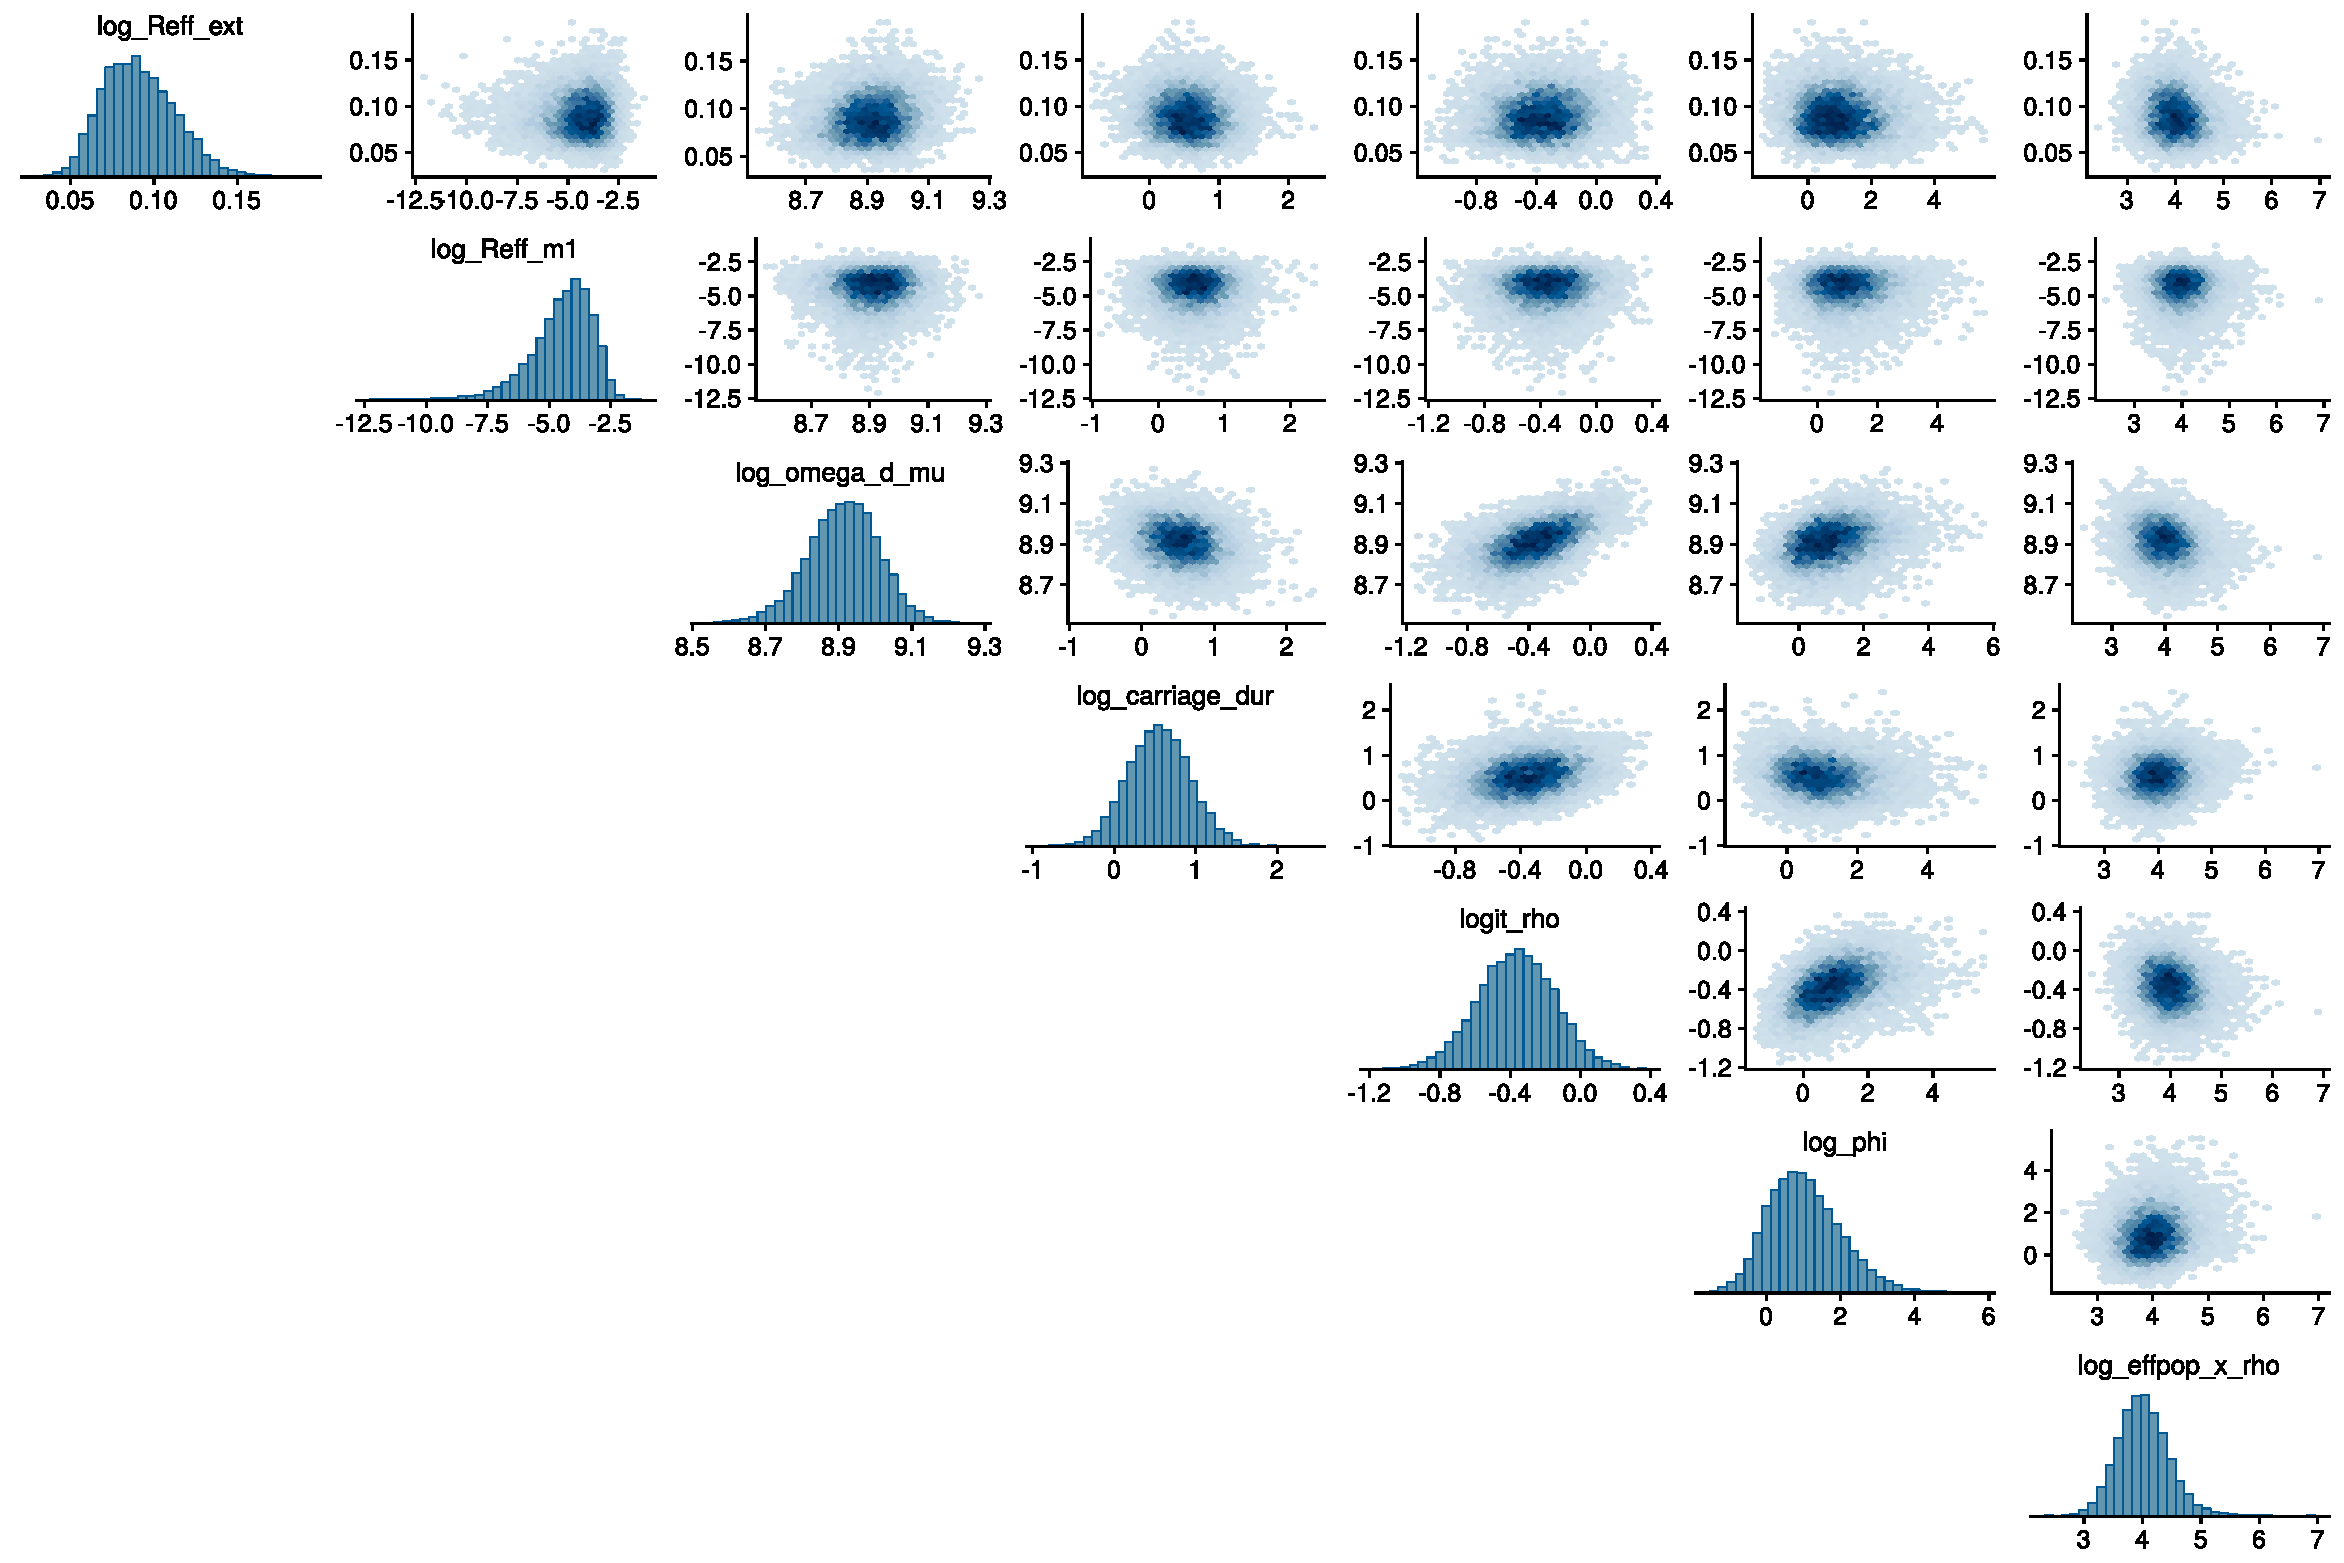
\includegraphics[width=\linewidth]{figures/sl_pairs_3}
	\caption{Marginal histograms and pairwise scatterplots of posterior samples for parameters for the SEIR model fit to the Sierra Leone Ebola dataset using the estimation scale in Table \ref{tab:seir_params_est3}. The parameters on the estimation scales in this figure and their interpretations are provided in Table \ref{tab:seir_params_est3}.} 
	\label{fig:slpairs3}
\end{figure}

\begin{figure}[!ht]
	\centering
%	\includegraphics[width=\linewidth]{figures/lib_pairs_est3}
	\caption{Marginal histograms and pairwise scatterplots of posterior samples for parameters for the SEIR model fit to the Liberia Ebola dataset using the estimation scale in Table \ref{tab:seir_params_est3}. The parameters on the estimation scales in this figure and their interpretations are provided in Table \ref{tab:seir_params_est3}.} 
	\label{fig:libpairs3}
\end{figure}

\section{Simulation Details and Additional Results for Section \ref{subsec:lna_coverage}}
\label{sec:lna_coverage_supplement}

\subsection{Simulation Setup and MCMC Details}
\label{subsec:lna_coverage_setup_details}

In this simulation, repeated for each of the three different regimes of population size and initial conditions given in Table \ref{tab:lna_coverage_sim}, we simulated 500 datasets according to the following procedure:
\begin{enumerate}
	\item Draw $ \log(R0 - 1),\ 1/\mu,\ \logit(\rho),\ \log(\phi) $ from the priors given in Table \ref{tab:lna_coverage_sim}.
	\item Simulate an outbreak, $ \bN|\btheta $, under SIR dynamics from the MJP via Gillespie's direct algorithm \cite{gillespie1976general}. If there were fewer than 15 cases, simulate another outbreak. 
	\item Simulate the observed incidence, $ \bY|\bN,\btheta $, as a negative binomial sample of the true incidence in each epoch, i.e., $ Y_\ell\sim\mr{Neg.Binomial(\rho(N_{SI}(t_\ell) - N_{SI}(t_{\ell-1})), \phi)} $. If the outbreak died off before epoch 15, the dataset was truncated at 15 observations (i.e., the dataset consisted of a series of case counts accrued during the outbreak along with a series of trailing zeros accrued after the outbreak died off). If the outbreak lasted longer than 50 epochs, the dataset was truncated at 50 observations
\end{enumerate}

We proceed to fit SIR models using the LNA, ODE, and MMTL approximations. Priors for model parameters were assigned as in Table \ref{tab:lna_coverage_sim}. Five MCMC chains per model were initialized at random values near the true parameters and run for 35,000 iterations per chain. The first 10,000 iterations used to warm up each chain and adaptively estimate the empirical covariance matrix to be used in the multivariate Gaussian random walk Metropolis--Hastings proposals for parameters. The empirical covariance matrix was initialized as 0.01 times an identity matrix. After the warm--up period, the empirical covariance matrix was frozen and the final 25,000 iterations from each chain were combined to form the final MCMC sample. Convergence was assessed using potential scale reduction factors (PSRFs) \cite{brooks1998general}, computed via the \texttt{coda} R package \cite{codapackage}. PSRFs were less than 1.05 in cases.

For models fit via the LNA and ODE approximations, the covariance matrix was adapted as in algorithm 4 of \cite{andrieu2008tutorial}. The gain factor sequence was $\gamma_n = 0.25(1 + 0.05n)^{0.50001}$, and a small nugget variance, equal to 0.00001 times an identity matrix, was added during the adaptation phase. The target acceptance rate used in the adaptation was 0.234. The models were implemented using the \text{stemr} R package \cite{stemr}.

Inference via the MMTL approximation within PMMH were fit using the \texttt{pomp} R package \cite{pompjss}. We used 500 particles in the PMMH algorithm. This choice was made to mitigate issues of particle degeneracy that occurred with fewer particles for some datasets. The time step for MMTL was set to 1/7, which, for example, corresponds to $ \tau $--leaping over one day increments given weekly incidence data. The MCMC was initialized in the same way as LNA and ODE models, but the empirical covariance matrix was adapted according to a different cooling schedule. The gain factor sequence provided by the package is $ \gamma_n = n^\alpha $, where the cooling term, $ \alpha $, was set to 0.999. For some of the datasets, the PMMH algorithm degenerated during the adaptive phase of the MCMC. If this was the case, the MCMC was restarted at a different set of random initial conditions. The posterior sample consisted of the combined samples from all five MCMC chains after discarding the initial samples from the adaptation phase.

\subsection{Additional Results}
\label{subsec:lna_coverage_additional_results}

\begin{sidewaystable}[!ht]
	\small
	\centering
	\begin{tabular}{lcccccc}
		\hline
		Method & Parameter & Coverage & PMD & 95\% CIW & ESS & Rel. GM ESS/CPU time \\ 
		\hline
		LNA & log(R0) & 0.93 & 0 (-0.51, 0.55) & 1.04 (0.83, 1.36) & 1340 (274, 4029) & 0.63 (0.13, 3.4) \\ 
		LNA & log($\mu$) & 0.95 & -0.01 (-0.5, 0.48) & 0.93 (0.74, 1.13) & 1024 (199, 3988) & 0.48 (0.1, 2.91) \\ 
		LNA & logit($\rho$) & 0.93 & -0.05 (-1.44, 0.56) & 1.18 (0.54, 2.86) & 1225 (316, 3941) & 0.62 (0.17, 4.05) \\ 
		LNA & log($\phi$) & 0.96 & 0 (-0.66, 0.71) & 1.35 (0.92, 2.22) & 2021 (687, 4535) & 1 (0.31, 3.53) \\ 
		MMTL & log(R0) & 0.95 & 0.03 (-0.48, 0.55) & 1.09 (0.88, 1.39) & 7483 (5453, 9197) & --- \\ 
		MMTL & log($\mu$) & 0.95 & -0.03 (-0.51, 0.45) & 0.92 (0.75, 1.09) & 7481 (5442, 9197) & --- \\ 
		MMTL & logit($\rho$) & 0.94 & -0.03 (-1, 0.61) & 1.17 (0.51, 2.98) & 6725 (4328, 8506) & --- \\ 
		MMTL & log($\phi$) & 0.96 & -0.02 (-0.69, 0.71) & 1.33 (0.91, 2.21) & 7486 (5405, 9215) & --- \\ 
		ODE & log(R0) & 0.89 & -0.03 (-0.76, 0.56) & 1.03 (0.65, 1.38) & 6438 (4956, 7650) & 185 (105, 340) \\ 
		ODE & log($\mu$) & 0.86 & 0.05 (-0.51, 0.79) & 0.91 (0.53, 1.2) & 6420 (4908, 7663) & 184 (103, 344) \\ 
		ODE & logit($\rho$) & 0.72 & 0.12 (-1.03, 1.37) & 1.25 (0.48, 2.94) & 6237 (4346, 7556) & 203 (111, 401) \\ 
		ODE & log($\phi$) & 0.75 & -0.25 (-1.64, 0.54) & 1.25 (0.88, 2.11) & 6529 (5459, 7778) & 189 (116, 340) \\ 
		\hline
	\end{tabular}
	\caption{Detailed small population (N = 10,000) regime results for the coverage simulation presented in Section \ref{subsec:lna_coverage}. Models were fit via the linear noise approximation (LNA), multinomial modified $ \tau $--leaping (MMTL) within particle marginal Metropolis--Hastings, and deterministic ordinary differential equations (ODE). $ R_0 $ is the basic reproductive number of an outbreak, $ \mu $ is the recovery rate, $ \rho $ is the negative binomial case detection probability, $ \phi $ is the negative binomial over--dispersion parameter. We report the coverage rates of 95\% Bayesian credible intervals along with 50\% (2.5\%, 97.5\%) quantiles of posterior median deviations (PMD), 95\% credible interval widths (CIW), effective sample size (ESS), and relative geometric mean effective sample size per CPU time (Rel. GM ESS/CPU time).}
\end{sidewaystable}	

\begin{sidewaystable}[!ht]
	\small
	\centering
	\begin{tabular}{lcccccc}
		\hline
		Method & Parameter & Coverage & PMD & 95\% CIW & ESS & Rel. GM ESS/CPU time \\ 
		\hline
		LNA & log(R0) & 0.93 & -0.03 (-0.5, 0.49) & 0.93 (0.66, 1.28) & 2158 (397, 4981) & 0.67 (0.16, 3) \\ 
		LNA & log($\mu$) & 0.93 & 0.01 (-0.43, 0.41) & 0.83 (0.58, 1.07) & 1919 (307, 5276) & 0.63 (0.12, 3.05) \\ 
		LNA & logit($\rho$) & 0.95 & -0.01 (-1, 0.5) & 1.13 (0.47, 2.81) & 1704 (439, 4636) & 0.61 (0.18, 3.49) \\ 
		LNA & log($\phi$) & 0.94 & 0.01 (-0.57, 0.7) & 1.1 (0.79, 1.86) & 2916 (1179, 5442) & 1.02 (0.38, 3.1) \\ 
		MMTL & log(R0) & 0.95 & -0.01 (-0.46, 0.51) & 0.98 (0.67, 1.32) & 7284 (4713, 9107) & --- \\ 
		MMTL & log($\mu$) & 0.93 & -0.01 (-0.47, 0.37) & 0.82 (0.58, 1.05) & 7167 (4488, 8912) & --- \\ 
		MMTL & logit($\rho$) & 0.95 & -0.03 (-0.98, 0.56) & 1.09 (0.43, 2.96) & 6452 (3999, 8318) & --- \\ 
		MMTL & log($\phi$) & 0.94 & -0.02 (-0.59, 0.65) & 1.1 (0.79, 1.84) & 7096 (4640, 8999) & --- \\ 
		ODE & log(R0) & 0.86 & -0.02 (-0.56, 0.59) & 0.84 (0.52, 1.27) & 6592 (5213, 7771) & 187 (88, 354) \\ 
		ODE & log($\mu$) & 0.82 & -0.01 (-0.66, 0.47) & 0.73 (0.44, 1.07) & 6558 (5129, 7664) & 190 (87, 359) \\ 
		ODE & logit($\rho$) & 0.75 & -0.03 (-1.13, 0.85) & 0.88 (0.37, 2.75) & 6421 (5017, 7643) & 209 (107, 410) \\ 
		ODE & log($\phi$) & 0.82 & -0.17 (-1.36, 0.57) & 1.04 (0.78, 1.7) & 6637 (5452, 7755) & 193 (102, 365) \\ 
		\hline
	\end{tabular}
	\caption{Detailed medium population (N = 50,000) regime results for the coverage simulation presented in Section \ref{subsec:lna_coverage}. Models were fit via the linear noise approximation (LNA), multinomial modified $ \tau $--leaping (MMTL) within particle marginal Metropolis--Hastings, and deterministic ordinary differential equations (ODE). $ R_0 $ is the basic reproductive number of an outbreak, $ \mu $ is the recovery rate, $ \rho $ is the negative binomial case detection probability, $ \phi $ is the negative binomial over--dispersion parameter. We report the coverage rates of 95\% Bayesian credible intervals along with 50\% (2.5\%, 97.5\%) quantiles of posterior median deviations (PMD), 95\% credible interval widths (CIW), effective sample size (ESS), and relative geometric mean effective sample size per CPU time (Rel. GM ESS/CPU time).}
\end{sidewaystable}	

\begin{sidewaystable}[!ht]
	\small
	\centering
	\begin{tabular}{lcccccc}
		\hline
		Method & Parameter & Coverage & PMD & 95\% CIW & ESS & Rel. GM ESS/CPU time \\ 
		\hline
		LNA & log(R0) & 0.95 & -0.01 (-0.38, 0.51) & 0.77 (0.47, 1.24) & 3248 (638, 6127) & 1.13 (0.22, 3.99) \\ 
		LNA & log($\mu$) & 0.95 & 0.01 (-0.44, 0.33) & 0.67 (0.4, 1.02) & 3134 (499, 6038) & 1.12 (0.18, 3.95) \\ 
		LNA & logit($\rho$) & 0.93 & 0.01 (-0.8, 0.57) & 0.99 (0.35, 2.66) & 2514 (572, 5905) & 1.03 (0.24, 4.71) \\ 
		LNA & log($\phi$) & 0.95 & 0 (-0.44, 0.54) & 0.94 (0.67, 1.5) & 3987 (2201, 6184) & 1.63 (0.71, 3.95) \\ 
		MMTL & log(R0) & 0.93 & 0.03 (-0.38, 1.04) & 0.8 (0.31, 1.27) & 7030 (3789, 8915) & --- \\ 
		MMTL & log($\mu$) & 0.94 & -0.02 (-0.46, 0.32) & 0.65 (0.38, 0.98) & 6858 (3602, 8871) & --- \\ 
		MMTL & logit($\rho$) & 0.92 & 0.01 (-0.7, 0.65) & 0.95 (0.34, 2.64) & 6166 (3282, 7906) & --- \\ 
		MMTL & log($\phi$) & 0.95 & -0.03 (-0.51, 0.52) & 0.94 (0.66, 1.5) & 6266 (3735, 8960) & --- \\ 
		ODE & log(R0) & 0.89 & -0.01 (-0.37, 0.55) & 0.65 (0.36, 1.22) & 6828 (5566, 8025) & 193 (104, 417) \\ 
		ODE & log($\mu$) & 0.89 & 0 (-0.49, 0.34) & 0.55 (0.3, 1) & 6815 (5520, 7877) & 198 (105, 428) \\ 
		ODE & logit($\rho$) & 0.84 & -0.01 (-0.78, 0.68) & 0.74 (0.27, 2.62) & 6575 (5219, 7838) & 210 (118, 486) \\ 
		ODE & log($\phi$) & 0.91 & -0.08 (-0.59, 0.46) & 0.9 (0.64, 1.44) & 6721 (5571, 7683) & 209 (117, 413) \\ 
		\hline
	\end{tabular}
	\caption{Detailed large population (N = 250,000) regime results for the coverage simulation presented in Section \ref{subsec:lna_coverage}. Models were fit via the linear noise approximation (LNA), multinomial modified $ \tau $--leaping (MMTL) within particle marginal Metropolis--Hastings, and deterministic ordinary differential equations (ODE). $ R_0 $ is the basic reproductive number of an outbreak, $ \mu $ is the recovery rate, $ \rho $ is the negative binomial case detection probability, $ \phi $ is the negative binomial over--dispersion parameter. We report the coverage rates of 95\% Bayesian credible intervals along with 50\% (2.5\%, 97.5\%) quantiles of posterior median deviations (PMD), 95\% credible interval widths (CIW), effective sample size (ESS), and relative geometric mean effective sample size per CPU time (Rel. GM ESS/CPU time).}
\end{sidewaystable}	

\newpage
\begin{table}[!ht]
	\small
	\centering
	\begin{tabular}{lccc}
		Population size & ODE & LNA & MMTL \\ 
		\hline
		10,000 & 0.39 (0.21, 0.62) & 21.73 (10.83, 37.74) & 85.23 (42.31, 152.48) \\ 
		50,000& 0.42 (0.23, 0.62) & 32.27 (13.4, 55.8) & 88.36 (38.63, 153.54) \\ 
		250,000 & 0.45 (0.25, 0.78) & 33.08 (12.56, 70.86) & 87.4 (39.8, 166.87) \\
		\hline
	\end{tabular}
	\caption{Median (2.5\%, 97.5\%) quantiles of run times, in minutes, for MCMC chains in the coverage simulation presented in Section \ref{subsec:lna_coverage}. Models were fit via the linear noise approximation (LNA), multinomial modified $ \tau $--leaping (MMTL) within particle marginal Metropolis--Hastings, and deterministic ordinary differential equations (ODE).}
\end{table}	

\newpage

\section{Supplementary Simulations with Fixed Parameters}
\label{sec:lna_fixedpar_coverage}

\subsection{Simulation Setup}
\label{subsec:lna_fixedpar_setup}

The simulations presented in this section supplement the results of Section \ref{subsec:lna_coverage} in assessing the statistical and computation performance of the LNA approximation vis--a--vis the ODE and MMTL approximations. In contrast to the previous coverage simulation, here we will fix the model parameters to one of four regimes, presented in Table \ref{tab:lna_supplementary_coverage_sim}, that are characterized by either fast or moderate outbreak dynamics, and high or low detection probability. In each setting, we simulated 500 outbreaks from a MJP with SIR dynamics in a population of 50,000 individuals, five of whom were initially infected and the rest of whom were susceptible. The observed incidence in each epoch was a negative binomial sample of the true incidence. Outbreaks for which the number of observed cases was less than 25 were re--simulated. MCMC chains were tuned and SIR models were fit via the LNA, ODE, and MMTL approximations as described in Section \ref{subsec:lna_coverage_setup_details}. The initial comparment volumes were fixed at the true values. The models were fit using diffuse priors, also presented in Table \ref{tab:lna_supplementary_coverage_sim}. We caution that the priors used in this exercise are perhaps unreasonably diffuse, particularly in the context of epidemic modeling where prior information is often available, and that we expect credible intervals will be overly wide as a result (we would still expect nominal coverage to be incorrect, even under tighter priors, since the datasets were simulated under fixed parameter regimes).

\subsection{Results}
\label{subsec:lna_fixedpar_sim_results}

Coverage for credible intervals of ODE models tended to fall below nominal levels in spite of the bias towards wide intervals due to the diffusivity of the priors. This was particularly the case in parameter regimes 1 and 3, where the basic reproductive number was lower (and hence the simulated outbreak trajectories further from their thermodynamic limits). In these parameter regimes, coverage was particularly poor due as estimates of the outbreak dynamics tended to be farther from their true values and credible intervals were too tight and did not properly account for uncertainty about the parameter estimates, particularly those governing the measurement process. Coverage levels for models fit via the LNA and MMTL approximations exceeded their nominal levels as expected. 

ODE models remained the most computationally performant. However, in this exercise, the LNA substantially outperformed the MMTL approximation within PMMH in terms of ESS and ESS per CPU time. We believe this is largely attributable to the diffusivity of the priors, which not only fail to regularize the posterior, but likely pull it towards unreasonable regions of the parameter space. As a general comment, we would strongly caution practitioners against adopting such priors more broadly. While it may seem appealing to adopt such diffuse priors in pursuit of being "agnostic" to the underlying outbreak dynamics, one of the very good reasons for working within the Bayesian paradigm in this context is that we have quite a bit of prior information regarding the outbreak dynamics and reasonable ranges for the case detection probability. For example, we often have historic examples of outbreaks in similar settings that we can look to in specifying priors about the basic reproductive number.

\begin{table}[!ht]
	\label{tab:lna_supplementary_coverage_sim}
	\caption{Parameter regimes under which datasets were simulated and priors used to fit SIR models. Five hundred datasets were simulated for each of the parameter regimes  from a MJP with SIR dynamics. $ R0 = \beta N / \mu $ is the basic reproductive number and $ \mu $ is the recovery rate. The observed incidence was a negative binomial sample of the true incidence in each inter--observation interval with case detection probability $ \rho $ and overdispersion parameter $ \phi $.}\footnotesize
	\centering
	\begin{tabular}{lcccc}
		& \textbf{Regime 1} & \textbf{Regime 2} & \textbf{Regime 3} & \textbf{Regime 4} \\
		& \makecell{Low R0/Low $ \rho $} & \makecell{High R0/Low $ \rho $} & \makecell{Low R0/High $ \rho $} & \makecell{High R0/High $ \rho $} \\
		\hline
		\textbf{R0} & 1.75 & 3.25 & 1.75 & 3.25 \\ 
		$ \bs{\rho} $ & 0.25 & 0.25 & 0.75 & 0.75 \\
		$ \mu $ & 1 & 0.4 & 1 & 0.4 \\
		$ \phi $ & 5 & 5 & 5 & 5\\
		\hline
		&&&
	\end{tabular} 
	
	\begin{tabular}{cllc}
		\textbf{Parameter} & \textbf{Interpretation} & \textbf{Prior} & \textbf{Median (95\% Interval)} \\ \hline
		$ R0-1 $ & Basic reproduction \# - 1 & LogCauchy(0.4, 1) & $ \implies R0 = $ 2.50 (1.00, 4.9$ \times 10^5$) \\ 
		$ 1/\mu $ & Mean infectious period & LogCauchy(-0.7, 1)& 1.43 ($ 4.3\times 10^{-6},\ 4.7\times 10^5 $) \\
		$ \rho $ & Mean case detection prob. & Unif(0, 1) & 0.5 (0.025, 0.975) \\
		$ \phi $ & Neg.Binom. overdispersion & LogCauchy(1.5,1) & 4.48 (1.4$ \times 10^{-5},\ 1.5\times10^6 $)\\
		\hline
	\end{tabular}
\end{table}

\subsection{Results}
\label{subsec:lna_fixedpar_results}


\begin{sidewaystable}[ht]
	\small
	\centering
	\begin{tabular}{lcccccc}
		\hline
		Method & Parameter & Coverage & PMD & 95\% CIW & ESS & Rel. GM ESS/CPU time \\ 
		\hline
		LNA & log(R0) & 0.99 & 0.23 (-0.33, 0.85) & 1.9 (1.2, 3.49) & 1200 (251, 2508) & 19.1 (2.7, 76.4) \\ 
		LNA & $\log(\mu)$ & 0.98 & -0.21 (-0.81, 0.28) & 1.73 (1.04, 3.42) & 1086 (228, 2295) & 27.9 (3.7, 100.5) \\ 
		LNA & $\logit(\rho)$ & 0.98 & -0.06 (-0.46, 0.4) & 1.07 (0.73, 1.67) & 1233 (360, 2180) & 8.22 (2.03, 21.4) \\ 
		LNA & $\log(\phi)$ & 0.98 & 0.01 (-0.51, 0.74) & 1.32 (1.17, 1.71) & 2950 (1145, 4334) & 10.8 (2.1, 30.0) \\ 
		MMTL & log(R0) & 0.99 & 0.22 (-0.86, 0.87) & 4.4 (1.92, 53.26) & 232 (110, 445) & --- \\ 
		MMTL & $\log(\mu)$ & 1.00 & -0.22 (-0.79, 0.52) & 2.02 (1.26, 3.63) & 125 (58, 283) & --- \\ 
		MMTL & $\logit(\rho)$ & 0.99 & -0.06 (-0.47, 0.48) & 1.21 (0.83, 1.72) & 492 (258, 874) & --- \\ 
		MMTL & $\log(\phi)$ & 0.97 & -0.01 (-0.54, 0.71) & 1.32 (1.16, 1.72) & 942 (541, 1791) & --- \\ 
		ODE & log(R0) & 0.84 & 0.3 (-0.77, 2.43) & 1.78 (1.12, 5.93) & 3364 (252, 6513) & 3894 (169, 13949) \\ 
		ODE & $\log(\mu)$ & 0.78 & -0.24 (-2.57, 0.7) & 1.56 (0.93, 5.81) & 3307 (243, 6489) & 6454 (277.52, 15693) \\ 
		ODE & $\logit(\rho)$ & 0.78 & -0.08 (-0.67, 0.79) & 0.77 (0.51, 1.52) & 5225 (2398, 6933) & 2500 (869, 5719) \\ 
		ODE & $\log(\phi)$ & 0.94 & -0.1 (-0.73, 0.57) & 1.26 (1.14, 1.54) & 5702 (2768, 6991) & 1451 (532, 3117) \\ 
		\hline
	\end{tabular}
	\caption{Detailed results for the fixed parameter  simulation in which outbreaks and datasets were simulated under parameter regime 1, characterized by slow outbreak dynamics (R0 = 1.75) and low mean case detection probability ($ \rho=0.25 $). Models were fit via the linear noise approximation (LNA), multinomial modified $ \tau $--leaping (MMTL) within particle marginal Metropolis--Hastings, and deterministic ordinary differential equations (ODE). $ R_0 $ is the basic reproductive number of an outbreak, $ \mu $ is the recovery rate, $ \rho $ is the negative binomial case detection probability, $ \phi $ is the negative binomial over--dispersion parameter. We report the coverage rates of 95\% Bayesian credible intervals along with 50\% (2.5\%, 97.5\%) quantiles of posterior median deviations (PMD), 95\% credible interval widths (CIW), effective sample size (ESS), and relative geometric mean effective sample size per CPU time (Rel. GM ESS/CPU time).}
\end{sidewaystable}

\begin{sidewaystable}[ht]
	\small
	\centering
	\begin{tabular}{lcccccc}
		\hline
		Method & Parameter & Coverage & PMD & 95\% CIW & ESS & Rel. GM ESS/CPU time \\ 
		\hline
		LNA & log(R0) & 0.99 & -0.35 (-0.87, -0.05) & 2.01 (1.42, 3.03) & 1551 (399, 3065) & 64.2 (10.3, 265.1) \\ 
		LNA & $\log(\mu)$ & 0.99 & 0.34 (0.09, 0.8) & 1.9 (1.34, 2.92) & 1431 (368, 2865) & 23.8 (5.0, 101.7) \\ 
		LNA & $\logit(\rho)$ & 0.94 & 0.12 (-0.23, 0.55) & 1.02 (0.73, 1.71) & 1354 (509, 2357) & 13.1 (3.2, 40.6) \\ 
		LNA & $\log(\phi)$ & 0.96 & 0.02 (-0.53, 0.81) & 1.38 (1.25, 1.76) & 3286 (1756, 4442) & 19.5 (6.3, 50.5) \\ 
		MMTL & log(R0) & 0.99 & -0.41 (-1.11, -0.08) & 13.94 (2.95, 55.97) & 132 (31, 314) & --- \\ 
		MMTL & $\log(\mu)$ & 0.99 & 0.4 (0.12, 0.99) & 2.74 (2.13, 3.69) & 213 (90, 1944) & --- \\ 
		MMTL & $\logit(\rho)$ & 0.90 & 0.18 (-0.18, 0.64) & 1.78 (1.1, 2.73) & 375 (171, 737) & --- \\ 
		MMTL & $\log(\phi)$ & 0.97 & -0.03 (-0.59, 0.78) & 1.42 (1.25, 2) & 586 (315, 993) & --- \\ 
		ODE & log(R0) & 0.99 & -0.22 (-0.84, 0.65) & 1.85 (1.31, 3.58) & 3979 (1875, 5747) & 9412 (2368, 34873) \\ 
		ODE & $\log(\mu)$ & 0.98 & 0.21 (-0.78, 0.8) & 1.72 (1.21, 3.53) & 3976 (1851, 5752) & 3824 (9812, 12367) \\ 
		ODE & $\logit(\rho)$ & 0.85 & 0.05 (-0.34, 0.52) & 0.71 (0.5, 1.08) & 5024 (2846, 6390) & 2753 (1205, 6858) \\ 
		ODE & $\log(\phi)$ & 0.95 & -0.03 (-0.64, 0.67) & 1.33 (1.23, 1.6) & 5634 (4377, 6661) & 2027 (995, 4479) \\ 
		\hline
	\end{tabular}
	\caption{Detailed results for the fixed parameter  simulation in which outbreaks and datasets were simulated under parameter regime 2, characterized by fast outbreak dynamics (R0 = 3.25) and low mean case detection probability ($ \rho = 0.25 $). Models were fit via the linear noise approximation (LNA), multinomial modified $ \tau $--leaping (MMTL) within particle marginal Metropolis--Hastings, and deterministic ordinary differential equations (ODE). $ R_0 $ is the basic reproductive number of an outbreak, $ \mu $ is the recovery rate, $ \rho $ is the negative binomial case detection probability, $ \phi $ is the negative binomial over--dispersion parameter. We report the coverage rates of 95\% Bayesian credible intervals along with 50\% (2.5\%, 97.5\%) quantiles of posterior median deviations (PMD), 95\% credible interval widths (CIW), effective sample size (ESS), and relative geometric mean effective sample size per CPU time (Rel. GM ESS/CPU time).}
\end{sidewaystable}

\begin{sidewaystable}[ht]
	\small
	\centering
	\begin{tabular}{lcccccc}
		\hline
		Method & Parameter & Coverage & PMD & 95\% CIW & ESS & Rel. GM ESS/CPU time \\ 
		\hline
		LNA & log(R0) & 0.96 & 0.26 (-0.22, 0.93) & 1.68 (1.01, 3.21) & 1354 (198, 3054) & 16.0 (1.6, 70.2) \\ 
		LNA & $\log(\mu)$ & 0.96 & -0.23 (-0.85, 0.16) & 1.49 (0.84, 3.23) & 1210 (191, 2931) & 25.1 (2.8, 83.6) \\ 
		LNA & $\logit(\rho)$ & 0.99 & -0.2 (-0.96, 0.84) & 3.1 (1.61, 4.6) & 935 (393, 1893) & 6.9 (2.4, 18.7) \\ 
		LNA & $\log(\phi)$ & 0.97 & 0.02 (-0.52, 0.67) & 1.25 (1.12, 1.52) & 2851 (1425, 4283) & 13.4 (4.3, 31.6) \\ 
		MMTL & log(R0) & 0.99 & 0.24 (-0.48, 0.96) & 2.49 (1.44, 36.95) & 313 (139, 634) & --- \\ 
		MMTL & $\log(\mu)$ & 0.99 & -0.24 (-0.87, 0.24) & 1.75 (1, 3.44) & 141 (57, 359) & --- \\ 
		MMTL & $\logit(\rho)$ & 1.00 & -0.2 (-0.93, 0.86) & 3.48 (2.04, 4.99) & 439 (244, 711) & --- \\ 
		MMTL & $\log(\phi)$ & 0.97 & -0.02 (-0.53, 0.64) & 1.25 (1.12, 1.56) & 723 (372, 1376) & --- \\ 
		ODE & log(R0) & 0.79 & 0.34 (-0.41, 2.6) & 1.52 (0.95, 5.73) & 3688 (285, 6453) & 2951 (127, 10756.39) \\ 
		ODE & $\log(\mu)$ & 0.77 & -0.28 (-2.73, 0.36) & 1.31 (0.8, 5.69) & 3650 (263, 6457) & 5349 (177, 14237) \\ 
		ODE & $\logit(\rho)$ & 0.80 & -0.19 (-1.41, 1.57) & 2.27 (0.9, 4.66) & 3418 (1896, 5721) & 1767 (704, 4279) \\ 
		ODE & $\log(\phi)$ & 0.91 & -0.15 (-0.75, 0.48) & 1.16 (1.08, 1.34) & 5787 (2679, 7035) & 1754 (640, 4124) \\ 
		\hline
	\end{tabular}
	\caption{Detailed results for the fixed parameter simulation in which outbreaks and datasets were simulated under parameter regime 3, characterized by slow outbreak dynamics (R0 = 1.75) and high mean case detection probability ($ \rho = 0.75 $). Models were fit via the linear noise approximation (LNA), multinomial modified $ \tau $--leaping (MMTL) within particle marginal Metropolis--Hastings, and deterministic ordinary differential equations (ODE). $ R_0 $ is the basic reproductive number of an outbreak, $ \mu $ is the recovery rate, $ \rho $ is the negative binomial case detection probability, $ \phi $ is the negative binomial over--dispersion parameter. We report the coverage rates of 95\% Bayesian credible intervals along with 50\% (2.5\%, 97.5\%) quantiles of posterior median deviations (PMD), 95\% credible interval widths (CIW), effective sample size (ESS), and relative geometric mean effective sample size per CPU time (Rel. GM ESS/CPU time).}
\end{sidewaystable}

\begin{sidewaystable}[ht]
	\small
	\centering
	\begin{tabular}{lcccccc}
		\hline
		Method & Parameter & Coverage & PMD & 95\% CIW & ESS & Rel. GM ESS/CPU time \\ 
		\hline
		LNA & log(R0) & 1.00 & -0.27 (-0.68, 0.04) & 1.7 (1.24, 2.64) & 2217 (504, 4142) & 68.6 (10.0, 342.8) \\ 
		LNA & $\log(\mu)$ & 1.00 & 0.25 (-0.01, 0.62) & 1.62 (1.18, 2.63) & 2014 (493, 3894) & 26.4 (4.7, 85.4) \\ 
		LNA & $\logit(\rho)$ & 0.98 & 0.25 (-0.58, 1.35) & 3.49 (2.06, 4.63) & 1290 (563, 2572) & 14.8 (4.9, 59.9) \\ 
		LNA & $\log(\phi)$ & 0.96 & 0.03 (-0.52, 0.76) & 1.31 (1.2, 1.62) & 3506 (1910, 4689) & 27.0 (11.2, 66.1) \\ 
		MMTL & log(R0) & 1.00 & -0.35 (-0.93, -0.04) & 13.37 (1.83, 46.16) & 181 (48, 409) & --- \\ 
		MMTL & $\log(\mu)$ & 1.00 & 0.33 (0.06, 0.83) & 2.65 (1.61, 3.72) & 272 (128, 1994) & --- \\ 
		MMTL & $\logit(\rho)$ & 0.96 & 0.4 (-0.49, 1.57) & 4.49 (3.15, 7.21) & 309 (133, 545) & --- \\ 
		MMTL & $\log(\phi)$ & 0.97 & -0.06 (-0.63, 0.64) & 1.62 (1.26, 2.61) & 457 (213, 848) & --- \\ 
		ODE & log(R0) & 0.99 & -0.18 (-0.78, 0.84) & 1.67 (1.14, 3.73) & 4463 (1987, 6336) & 7879 (1915, 29567) \\ 
		ODE & $\log(\mu)$ & 0.99 & 0.18 (-0.99, 0.73) & 1.56 (1.07, 3.67) & 4424 (1952, 6312) & 3254 (867, 8316) \\ 
		ODE & $\logit(\rho)$ & 0.89 & 0.13 (-0.86, 1.71) & 2.59 (1.1, 4.57) & 3378 (1971, 5315) & 2271 (916, 7206) \\ 
		ODE & $\log(\phi)$ & 0.94 & -0.07 (-0.66, 0.62) & 1.26 (1.17, 1.48) & 5697 (4518, 6929) & 2490 (1211, 6558) \\ 
		\hline
	\end{tabular}
	\caption{Detailed results for the fixed parameter simulation in which outbreaks and datasets were simulated under parameter regime 4, characterized by fast outbreak dynamics (R0 = 3.25) and high mean case detection probability ($ \rho = 0.75 $). Models were fit via the linear noise approximation (LNA), multinomial modified $ \tau $--leaping (MMTL) within particle marginal Metropolis--Hastings, and deterministic ordinary differential equations (ODE). $ R_0 $ is the basic reproductive number of an outbreak, $ \mu $ is the recovery rate, $ \rho $ is the negative binomial case detection probability, $ \phi $ is the negative binomial over--dispersion parameter. We report the coverage rates of 95\% Bayesian credible intervals along with 50\% (2.5\%, 97.5\%) quantiles of posterior median deviations (PMD), 95\% credible interval widths (CIW), effective sample size (ESS), and relative geometric mean effective sample size per CPU time (Rel. GM ESS/CPU time).}
\end{sidewaystable}

\begin{table}[ht]
	\centering
	\begin{tabular}{lccc}
		\hline
		Parameter Regime & ODE & LNA & MMTL \\ 
		\hline
		Regime 1& 0.3 (0.21, 0.34) & 19.93 (14.96, 28.21) & 62.85 (54.16, 83.94) \\ 
		Regime 2& 0.28 (0.17, 0.36) & 14.41 (11.33, 20.43) & 48.89 (35.47, 67.2) \\ 
		Regime 3& 0.31 (0.2, 0.4) & 19.47 (15.57, 28.28) & 62.09 (55.75, 83.89) \\ 
		Regime 4& 0.28 (0.17, 0.36) & 14.66 (11.43, 20.58) & 49.04 (35.72, 67.53) \\ 
		\hline
	\end{tabular}
	\caption{Median (2.5\%, 97.5\%) quantiles of run times, in minutes, for MCMC chains in fixed parameter coverage simulations. Models were fit via the linear noise approximation (LNA), multinomial modified $ \tau $--leaping (MMTL) within particle marginal Metropolis--Hastings, and deterministic ordinary differential equations (ODE). True parameter values are presented in Table \ref{tab:lna_supplementary_coverage_sim}. Parameter regimes 1 and 3 had slower outbreak dynamics (R0 = 1.75, vs. R0 = 3.25). Parameter regimes 3 and 4 had higher case detection rates ($ \rho = 0.75 $, vs $ \rho = 0.25 $).}
\end{table}

\section{LNA Implementation Details and LNA Model Vignettes}
\label{sec:lna_implementation_vignettes}